\documentclass[journal,12pt,twocolumn]{IEEEtran}

\usepackage{setspace}
\usepackage{gensymb}
\singlespacing
\usepackage[cmex10]{amsmath}

\usepackage{amsthm}
\usepackage{float}
\usepackage{mathrsfs}
\usepackage{txfonts}
\usepackage{stfloats}
\usepackage{bm}
\usepackage{cite}
\usepackage{cases}
\usepackage{subfig}

\usepackage{longtable}
\usepackage{multirow}

\usepackage{enumitem}
\usepackage{mathtools}
\usepackage{steinmetz}
\usepackage{tikz}
\usepackage{circuitikz}
\usepackage{verbatim}
\usepackage{tfrupee}
\usepackage[breaklinks=true]{hyperref}
\usepackage{graphicx}
\usepackage{tkz-euclide}

\usetikzlibrary{calc,math}
\usepackage{listings}
    \usepackage{color}                                            %%
    \usepackage{array}                                            %%
    \usepackage{longtable}                                        %%
    \usepackage{calc}                                             %%
    \usepackage{multirow}                                         %%
    \usepackage{hhline}                                           %%
    \usepackage{ifthen}                                           %%
    \usepackage{lscape}     
\usepackage{multicol}
\usepackage{chngcntr}

\DeclareMathOperator*{\Res}{Res}

\renewcommand\thesection{\arabic{section}}
\renewcommand\thesubsection{\thesection.\arabic{subsection}}
\renewcommand\thesubsubsection{\thesubsection.\arabic{subsubsection}}

\renewcommand\thesectiondis{\arabic{section}}
\renewcommand\thesubsectiondis{\thesectiondis.\arabic{subsection}}
\renewcommand\thesubsubsectiondis{\thesubsectiondis.\arabic{subsubsection}}


\hyphenation{op-tical net-works semi-conduc-tor}
\def\inputGnumericTable{}                                 %%

\lstset{
%language=C,
frame=single, 
breaklines=true,
columns=fullflexible
}
\begin{document}


\newtheorem{theorem}{Theorem}[section]
\newtheorem{problem}{Problem}
\newtheorem{proposition}{Proposition}[section]
\newtheorem{lemma}{Lemma}[section]
\newtheorem{corollary}[theorem]{Corollary}
\newtheorem{example}{Example}[section]
\newtheorem{definition}[problem]{Definition}

\newcommand{\BEQA}{\begin{eqnarray}}
\newcommand{\EEQA}{\end{eqnarray}}
\newcommand{\define}{\stackrel{\triangle}{=}}
\bibliographystyle{IEEEtran}
\raggedbottom
\setlength{\parindent}{0pt}
\providecommand{\mbf}{\mathbf}
\providecommand{\pr}[1]{\ensuremath{\Pr\left(#1\right)}}
\providecommand{\qfunc}[1]{\ensuremath{Q\left(#1\right)}}
\providecommand{\sbrak}[1]{\ensuremath{{}\left[#1\right]}}
\providecommand{\lsbrak}[1]{\ensuremath{{}\left[#1\right.}}
\providecommand{\rsbrak}[1]{\ensuremath{{}\left.#1\right]}}
\providecommand{\brak}[1]{\ensuremath{\left(#1\right)}}
\providecommand{\lbrak}[1]{\ensuremath{\left(#1\right.}}
\providecommand{\rbrak}[1]{\ensuremath{\left.#1\right)}}
\providecommand{\cbrak}[1]{\ensuremath{\left\{#1\right\}}}
\providecommand{\lcbrak}[1]{\ensuremath{\left\{#1\right.}}
\providecommand{\rcbrak}[1]{\ensuremath{\left.#1\right\}}}
\theoremstyle{remark}
\newtheorem{rem}{Remark}
\newcommand{\sgn}{\mathop{\mathrm{sgn}}}
\providecommand{\abs}[1]{\left\vert#1\right\vert}
\providecommand{\res}[1]{\Res\displaylimits_{#1}} 
\providecommand{\norm}[1]{\left\lVert#1\right\rVert}
%\providecommand{\norm}[1]{\lVert#1\rVert}
\providecommand{\mtx}[1]{\mathbf{#1}}
\providecommand{\mean}[1]{E\left[ #1 \right]}
\providecommand{\fourier}{\overset{\mathcal{F}}{ \rightleftharpoons}}
%\providecommand{\hilbert}{\overset{\mathcal{H}}{ \rightleftharpoons}}
\providecommand{\system}{\overset{\mathcal{H}}{ \longleftrightarrow}}
	%\newcommand{\solution}[2]{\textbf{Solution:}{#1}}
\newcommand{\solution}{\noindent \textbf{Solution: }}
\newcommand{\cosec}{\,\text{cosec}\,}
\providecommand{\dec}[2]{\ensuremath{\overset{#1}{\underset{#2}{\gtrless}}}}
\newcommand{\myvec}[1]{\ensuremath{\begin{pmatrix}#1\end{pmatrix}}}
\newcommand{\mydet}[1]{\ensuremath{\begin{vmatrix}#1\end{vmatrix}}}
\numberwithin{equation}{subsection}
\makeatletter
\@addtoreset{figure}{problem}
\makeatother
\let\StandardTheFigure\thefigure
\let\vec\mathbf
\renewcommand{\thefigure}{\theproblem}
\def\putbox#1#2#3{\makebox[0in][l]{\makebox[#1][l]{}\raisebox{\baselineskip}[0in][0in]{\raisebox{#2}[0in][0in]{#3}}}}
     \def\rightbox#1{\makebox[0in][r]{#1}}
     \def\centbox#1{\makebox[0in]{#1}}
     \def\topbox#1{\raisebox{-\baselineskip}[0in][0in]{#1}}
     \def\midbox#1{\raisebox{-0.5\baselineskip}[0in][0in]{#1}}
\vspace{3cm}
\title{CBSE Maths Questions 2007}
\author{Priyanka - EE21MTECH12002}
\maketitle
\newpage
\bigskip
\renewcommand{\thefigure}{\theenumi}
\renewcommand{\thetable}{\theenumi}
%
Get latex-tikz codes from 
%
\begin{lstlisting}
https://github.com/PeriPriyanka/cbsemathsquestions/2007/12/problems/questions
\end{lstlisting}
\section{Section-A}
\begin{enumerate}
\item If $\vec{A} =\myvec{2&-3\\3&4}$, show that $\vec{A}^2 - 6\vec{A} + 17\vec{I} = 0$. Hence find $\vec{A}^{-1}$
\item An urn contains 7 red and 4 blue balls. Two balls are drawn at random with replacement. Find the probability of getting
\begin{enumerate}
\item 2 red balls
\item 2 blue balls
\item one red and one blue ball
\end{enumerate} 
\item Using the properties of determinants, prove the following:
\begin{center}
$\begin{vmatrix}
a-b-c & 2a& 2a\\ 2b& b-c-a& 2b\\2c&2c&c-a-b 
\end{vmatrix}
= (a+b+c)^3$
\end{center}
\item A card is drawn at random from a well-shuffled pack of 52 cards. Find the probability that it is neither a ace or a king.
\item Evaluate the following integral:
\begin{center}
$ \int \displaystyle\frac{1+x^2}{1+x^4}\,dx $
\end{center}
\item Solve the following differential equation:
\begin{center}
$x \cos y dy=(xe^x\log x + e^x)$
\end{center}
\item Form the differential equations of the family of the curves $y = A\cos 2x + B\sin 2x$, where A and B are constants.
\item Solve the following differential equation:
\begin{center}
   $ \displaystyle\frac{dy}{dx} + 2y = 6e^x $
\end{center}
\item Evaluate:
\begin{center}
  $ \int \cos 4x\cos 3x\, dx $
\end{center}
\item Using the properties of definite integrals, prove the following:
\begin{center}
 $ \int_{0}^{\pi} \displaystyle\frac{x\tan x}{\sec x\cosec x}\, dx = \displaystyle\frac{\pi^2}{4} $
\end{center}
\item Evaluate: 
\begin{center}
    $ \int \displaystyle\frac{\sin x}{(1-\cos x)(2-\cos x)}\, dx $
\end{center} 
\item Find the value of k if the function
\begin{center}
   $ f(x) =
   \left\{
\begin{array}{ll}
      kx^2, & x\geq 1 \\
      4, & x <  1 
\end{array} \right. $
\text{is continuous at x = 1}
\end{center}

 \item Evalutate: 
 \begin{center}
   \[ \lim_{x\to\frac{\pi}{4}} \left(\displaystyle\frac{\sin x - \cos x}{x - \displaystyle\frac{\pi}{4}}\right) \]
 \end{center}
 
 \item Differentiate  $ \sin (x^2 + 1) $ with respect to x from first principle.

 \item Write the boolean expressions representing the following circuit and simplify the Boolean expression.
 \begin{figure}[H]
   \centering
   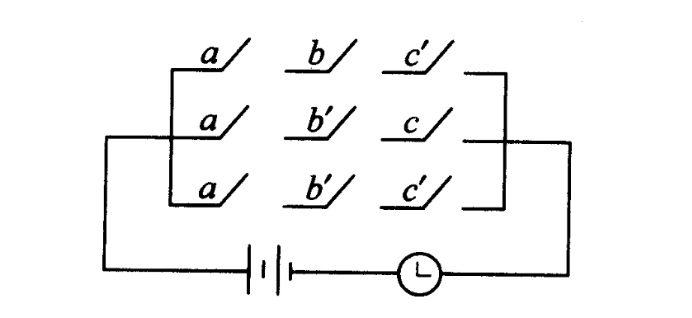
\includegraphics[width=10cm]{1.png}
\end{figure}

 \item Show that the following argument is valid:
 \begin{center}
    $ S_1 : p \vee q $  \\
   $ S_2 : p \sim q $ \\
    $ S : p \wedge q $ 
 \end{center}

 \item If y = $\sin(\log x)$, prove that
 \begin{center}
    $ x^2\displaystyle\frac{d^2y}{dx^2} + x\displaystyle\frac{dy}{dx} + y = 0$
 \end{center}

 \item Verify Rolle's theorem for the function $ f(x) = x^2-5x+4 $ on [1,4].

 \item Using matrices, solve the following system of equation:
 \begin{center}
    $ x+2y-3z=6 $   \\
     $ 3x+2y-2z=3 $   \\
     $ 2x-y+z=2 $ 
 \end{center}

 \item Using integration, find the are of the region enclosed between the circles $x^2+y^2=1$ and $(x-1)^2+y^2=1$. 

 \item Evaluate $ \int_{0}^{2} (x^2+2x+1)\, dx $ as limit of sum. 

 \item Find the point on the curve $x^2=8y $ which is nearest to the point (2,4).

 \item Show that a right circular cone of least curved surface and given volume has an altitude equal to $ \sqrt{2} $ times the radius of the base.
 \section{Section B}

 \item Find the projection of $\overrightarrow{\vec{b}}+\overrightarrow{\vec{c}}$ on $\overrightarrow{\vec{a}}$ where $\overrightarrow{\vec{a}}=2\hat{\vec{i}}-2\hat{\vec{j}}+\hat{\vec{k}} , \overrightarrow{\vec{b}}=\hat{\vec{i}}+2\hat{\vec{j}}-2\hat{\vec{k}}$ and $ \overrightarrow{\vec{c}}=2\hat{\vec{i}}-\hat{\vec{j}}+4\hat{\vec{k}}$

 \item Find the value of $\lambda$ which makes the vectors $\overrightarrow{\vec{a}}$,$\overrightarrow{\vec{b}}$ and $\overrightarrow{\vec{c}}$ coplanar, where $ \overrightarrow{\vec{a}}=2\hat{\vec{i}}-\hat{\vec{j}}+\hat{\vec{k}}$,$ \overrightarrow{\vec{b}}=\hat{\vec{i}}+2\hat{\vec{j}}-3\hat{\vec{k}}$ and $ \overrightarrow{\vec{c}}=3\hat{\vec{i}}-\lambda\hat{\vec{j}}+5\hat{\vec{k}}$

\item  A particle starting with initial velocity of 30 m/sec moves with a uniform acceleration of 9 m/sec$^2$. Find :
\begin{enumerate}
   \item the velocity of the particle after 6 seconds.
   \item how far it will go in 9 seconds.
   \item its velocity when is has traversed 150 m.
\end{enumerate}
\item Find the resultant of two velocities 4 m/sec and 6 m/sec inclined to one another at an angle of 120\degree.
\item A ball projected with a velocity of 28 m/sec has a horizontal range 40 m. Find the two angles of projection.
\item A body of weight 70 N is suspended by two strings of length 27 cm and 36 cm, fastened to two points in the same horizontal line 45 cm apart and is in equilibrium. Find the tensions in the strings.
\item The resultant of two unlike parallel forces of 18 N and 10 N act along a line at a distance of 12 cm from the line of action of the smaller force. Find the distance between the lines of action of two forces.
\item Find the equation of the plane which is perpendicular to the plane $5x + 3y + 6 z + 8 = 0$ and which contains the line of intersection of the planes $x + 2y + 3z - 4 = 0 $ and $2x + y - z + 5 = 0$.
\item Find the equation of the sphere which passing through the points $ (3, 0, 0), (0, -1, 0), (0, 0, -2)$ and and having the centre on the plane $3x + 2y + 4z = 1$.
\section{Section C}
\item Find the face value of a bill, discounted at 6\% per annum 146 days before the legal due date, if the banker's gain is Rs. 36.
\item A bill for Rs. 7650 was drawn on 8th March 2005 at 7 months. It was discounted on 18 May 2005 and the holder of the bill received Rs. 7497. What rate of interest did the banker charge ?
\item There are two bags I and II. Bag I contains 2 white and 3 red balls and Bag II contains 4 white and 5 red balls. One ball is drawn at random from one of the bags and is found to be red. Find the probability that it was drawn from bag II.
\item Find the mean $\mu$, variance $\sigma^2$ for the following probability distribution:
\begin{figure}[H]
   \centering
   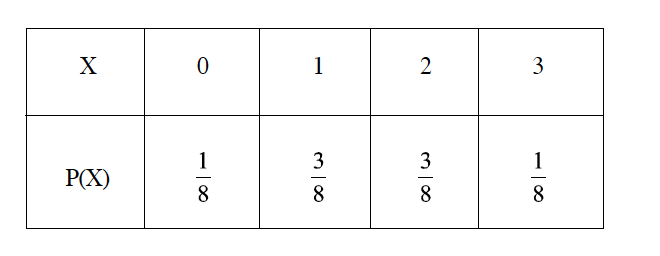
\includegraphics[width=10cm]{2.png}
\end{figure}
\item Find the binomial distribution for which the mean is 4 and variance 3.
\item A, B, C entered into a partnership investing Rs. 12000, Rs. 16000 and
Rs. 20000 respectively. A as working partner gets 10\% of the annual profit for
the same. After 5 months, B invested Rs. 2000 more while C withdrew Rs. 2000
after 8 months from the start of the business. Find the share of each in an
annual profit of Rs. 97000.
\item Find the present value of an annuity due of Rs. 700 per annum payable at the
beginning of each year for 2 years allowing interest 6\% per annum, compounded
annually.[Take $(1.06)^{-1} = 0.943$]
\item The total cost C(x), associated with the production and making x units of an item is given by
\begin{center}
   $C(x) = 0.005x^3 - 0.02x^2 + 30x + 5000 $ 
\end{center}
Find:
\begin{enumerate}
\item the average cost function.
\item the average cost of output of 10 units.
\item the marginal cost function.
\item the marginal cost when 3 units are produced.
\end{enumerate}
\item If a young man rides his motorcycle at 25 km/hour, he had to spend Rs. 2 per
km on petrol. If he rides at a faster speed of 40 km/hour, the petrol cost increases
at Rs. 5 per km. He has Rs. 100 to spend on petrol and wishes to find what is
the maximum distance he can travel within one hour. Express this as an LPP
and solve it graphically.
\end{enumerate}
\end{document}